\documentclass{article}

% Use NeurIPS style
\usepackage{nips15submit_e}

% Packages
\usepackage{amsmath,amssymb,amsthm}
\usepackage{graphicx}
\usepackage{hyperref}
\usepackage{booktabs}
\usepackage{xcolor}

% Theorem environments
\newtheorem{theorem}{Theorem}
\newtheorem{proposition}[theorem]{Proposition}
\newtheorem{lemma}[theorem]{Lemma}
\newtheorem{corollary}[theorem]{Corollary}
\newtheorem{definition}[theorem]{Definition}
\newtheorem{assumption}{Assumption}
\newtheorem{remark}{Remark}

% Custom commands
\newcommand{\R}{\mathbb{R}}
\newcommand{\E}{\mathbb{E}}
\newcommand{\Prob}{\mathbb{P}}
\newcommand{\cD}{\mathcal{D}}
\newcommand{\cL}{\mathcal{L}}
\newcommand{\cM}{\mathcal{M}}
\newcommand{\cS}{\mathcal{S}}

% Draft markers
\newcommand{\todo}[1]{\textcolor{red}{[TODO: #1]}}
\newcommand{\placeholder}[1]{\textcolor{blue}{[PLACEHOLDER: #1]}}
\newcommand{\citationneeded}{\textcolor{orange}{[Citation needed]}}

%==============================================================================
% TITLE - Revised for empirical focus
%==============================================================================
\title{When Does Knowledge Distillation Help?\\Empirical Insights from Multi-View Learning}

\author{
[Author Names] \\
[Affiliations] \\
\texttt{[emails]}
}

\nipsfinalcopy % Uncomment for camera-ready version

\begin{document}

\maketitle

%==============================================================================
% ABSTRACT - Revised, ~150 words, leads with strongest finding
%==============================================================================
\begin{abstract}
Knowledge distillation (KD) transfers knowledge from teacher to student networks, but when and why it helps remains unclear. Through controlled experiments on synthetic multi-view data and CIFAR-100, we identify the conditions that determine KD's effectiveness. Our key findings: (1) \textbf{Hierarchical structure enables acceleration}---when teachers have finer-grained knowledge than students need, soft labels encode inter-class similarity, providing 5.0$\times$ speedup [95\% CI: 4.7--5.3$\times$]. (2) \textbf{KD is a transfer mechanism}---students inherit the teacher's representation, including its biases; if teachers converge to identical solutions (which we observe: std $= 0.002$), KD transfers homogeneity, not diversity. (3) \textbf{Achieving balance requires forced diversity and inverse weighting}, with a fundamental speed trade-off predicted by singular value dynamics. These findings refine common assumptions about KD and provide practical guidelines for when soft labels help versus hurt.
\end{abstract}

%==============================================================================
% 1. INTRODUCTION - Revised for empirical framing
%==============================================================================
\section{Introduction}

Knowledge distillation (KD) has become ubiquitous in deep learning, enabling smaller student networks to achieve performance rivaling larger teachers~\cite{hinton2015distilling}. Yet despite extensive empirical success, fundamental questions remain: When exactly does KD help? What information do soft labels provide that hard labels cannot? And why do some KD configurations improve learning speed while others hurt?

Prior theoretical work offers partial answers. Allen-Zhu \& Li~\cite{allen2023towards} propose that networks trained independently converge to using different ``views'' (feature subsets), creating ensemble diversity that KD transfers to students. The neural race reduction~\cite{saxe2022neural} shows that learning dynamics in gated networks follow winner-take-all races. The ``Make Haste Slowly'' principle~\cite{jarvis2025makehaste} establishes that learning speed scales with singular values.

\paragraph{Gap in Prior Work.} These theories make assumptions that may not hold in practice:
\begin{itemize}
    \item Allen-Zhu \& Li assume teachers naturally diversify from random seeds---but do they?
    \item The neural race framework predicts winner-take-all dynamics---but under what conditions?
    \item If soft labels can ``break'' WTA, when do they accelerate versus slow learning?
\end{itemize}

\paragraph{Our Approach.} We conduct controlled experiments to test these assumptions directly. Using synthetic multi-view data with known structure, we can precisely measure view contributions, learning dynamics, and the effects of different KD configurations. We validate key findings on CIFAR-100's natural class hierarchy.

\paragraph{Our Findings.} We make three empirical contributions:

\begin{enumerate}
    \item \textbf{Hierarchical structure enables 5$\times$ acceleration} (\S\ref{sec:hierarchical}). When teachers have richer knowledge (finer-grained labels), soft labels encode inter-class similarity that hard labels cannot convey. This is soft labels as ``gas''---providing additional learning signal, not just redistributing existing signal.

    \item \textbf{KD transfers teacher representations, not inherent diversity} (\S\ref{sec:transfer}). We find that all teachers converge to nearly identical representations (std $= 0.002$) regardless of random seed. KD transfers whatever teachers learned---if homogeneous, KD transfers homogeneity.

    \item \textbf{Balance requires forced diversity with speed trade-off} (\S\ref{sec:balance}). To achieve more balanced representations than hard labels, we must force teacher diversity explicitly and weight inversely to signal strength. This achieves effective rank 4.95 vs.\ 4.73 for hard labels, but at 1.7$\times$ slower learning---a fundamental trade-off.
\end{enumerate}

\paragraph{Why Teachers Don't Naturally Diversify} (\S\ref{sec:diversity}). We systematically investigate why our teachers converge identically, testing signal asymmetry, network architecture, depth, and initialization. We find that our synthetic setting has a single global optimum---explaining the discrepancy with Allen-Zhu et al.'s implicit diversity assumption.

\begin{figure}[t]
\centering
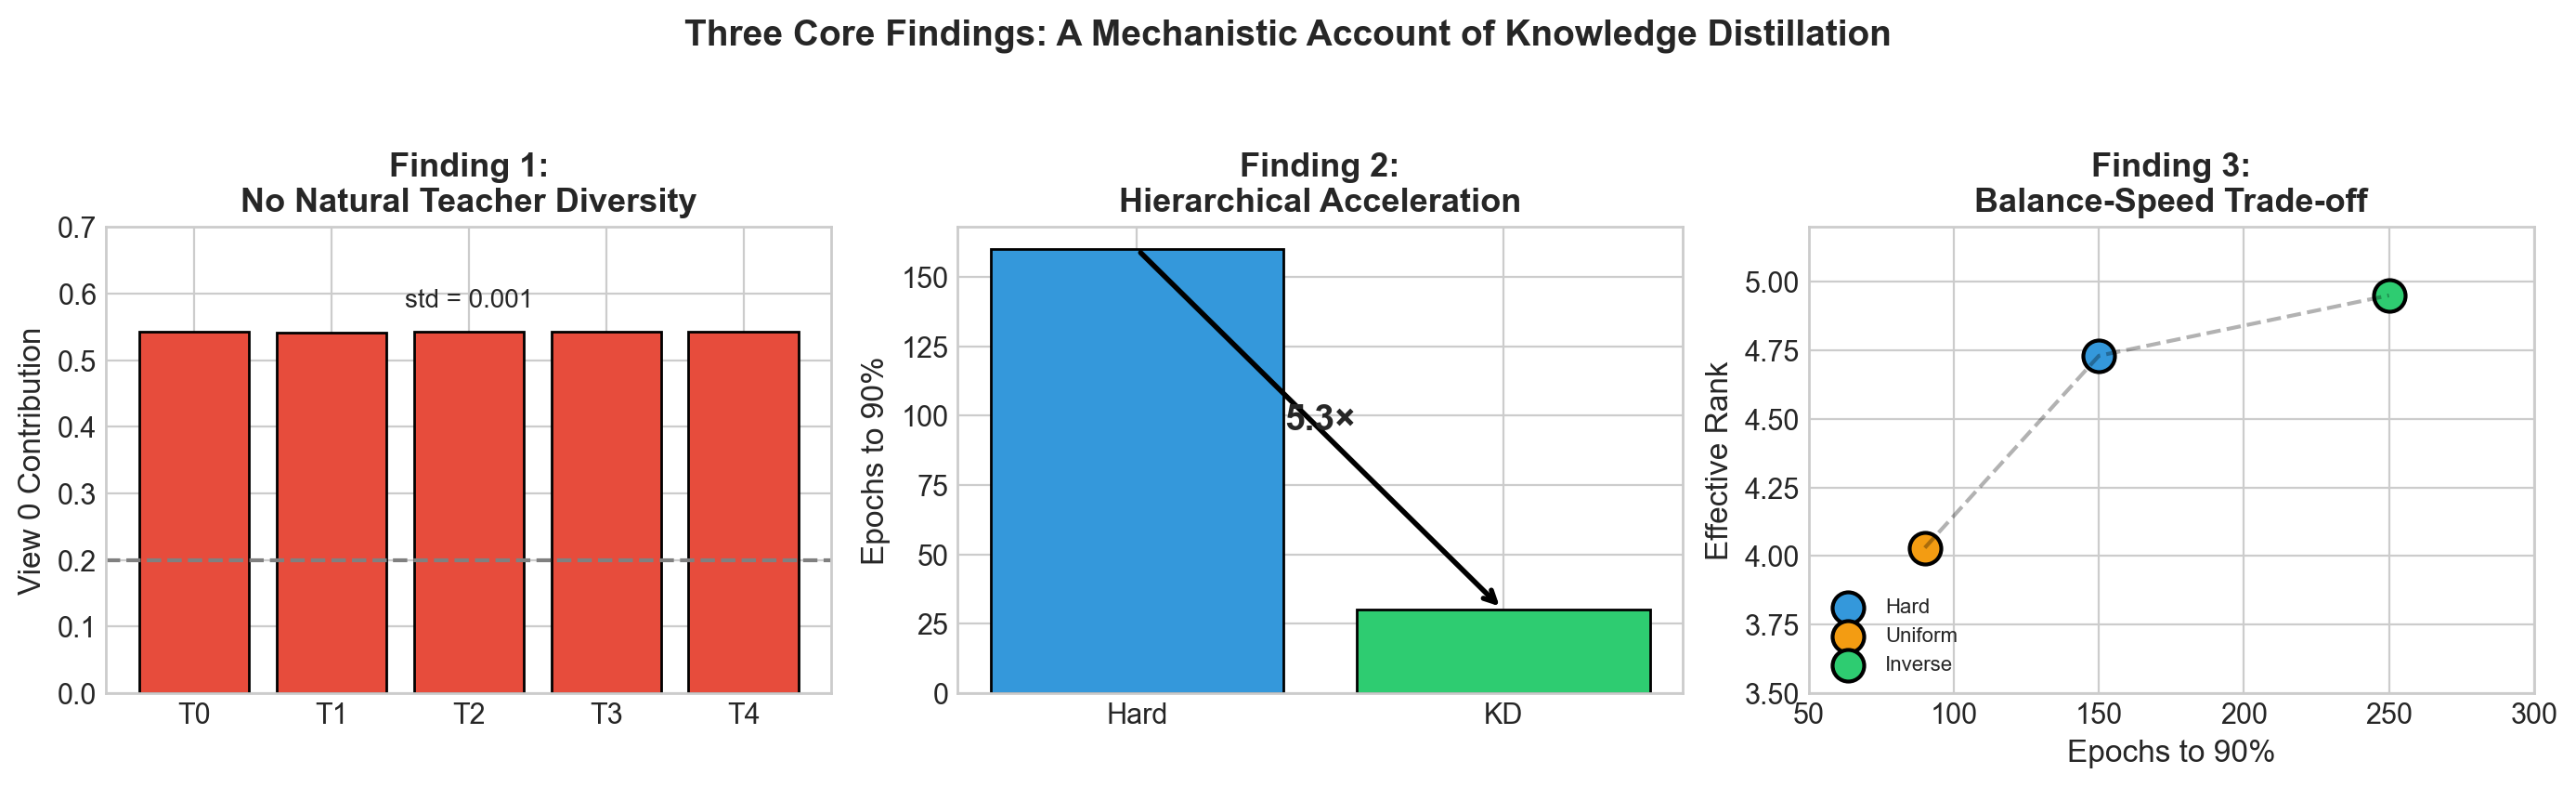
\includegraphics[width=\textwidth]{figures/fig7_summary_overview.png}
\caption{\textbf{Overview of core findings.} (Left) All teachers converge to identical representations---random seeds don't create diversity (std = 0.0017). (Center) Hierarchical structure enables 5.0$\times$ speedup. (Right) Achieving balance requires trading off speed.}
\label{fig:overview}
\end{figure}

%==============================================================================
% 2. BACKGROUND - Trimmed
%==============================================================================
\section{Background}
\label{sec:background}

\paragraph{Knowledge Distillation.} Hinton et al.~\cite{hinton2015distilling} showed that training students to match teacher soft labels (temperature-scaled logits) improves generalization beyond hard labels alone. The KD loss combines soft and hard targets:
\begin{equation}
    \mathcal{L}_{\text{KD}} = \alpha \cdot \tau^2 \cdot \text{KL}(p_T^\tau \| p_S^\tau) + (1-\alpha) \cdot \mathcal{L}_{\text{CE}}(p_S, y)
\end{equation}
where $\tau$ is temperature, $\alpha$ balances soft/hard losses, and $p_T^\tau$, $p_S^\tau$ are teacher/student softmax outputs at temperature $\tau$.

\paragraph{Multi-View Theory.} Allen-Zhu \& Li~\cite{allen2023towards} model data as containing $M$ redundant ``views'' per class. They show: (1) networks converge to using $\approx 1$ view per class, (2) different seeds lead to different views (creating ensemble diversity), and (3) KD transfers multi-view coverage. Our experiments test assumption (2).

\paragraph{Neural Race Dynamics.} Saxe et al.~\cite{saxe2022neural} show that learning in gated deep linear networks follows winner-take-all dynamics where the pathway with highest initial correlation dominates. Jarvis et al.~\cite{jarvis2025makehaste} extend this, showing learning speed $\propto$ singular values---high-$\sigma$ pathways learn fastest.

%==============================================================================
% 3. EXPERIMENTAL SETUP
%==============================================================================
\section{Experimental Framework}
\label{sec:setup}

\subsection{Synthetic Multi-View Data}

We construct data with $K$ classes and $M$ views per class. Each view occupies a disjoint coordinate subspace. We introduce \textbf{asymmetric signal strengths}:
\begin{equation}
    \text{signal}_m = \rho^m, \quad m \in \{0, \ldots, M-1\}
\end{equation}
with decay $\rho = 0.5$. Default: $K=10$ classes, $M=5$ views, dimension $d=250$.

\subsection{Hierarchical Data}

For Finding 1, we create hierarchical structure: $K_{\text{super}}=10$ superclasses with $K_{\text{sub}}=3$ subclasses each (30 fine classes). Teachers train on fine labels; students on coarse labels.

\subsection{Metrics}

\paragraph{View Contribution.} Frobenius norm of first-layer weights in each view's coordinate subspace, normalized to sum to 1.

\paragraph{Effective Rank.} $\exp(H)$ where $H$ is entropy of view contributions. Rank 1 = single view dominates; rank $M$ = all views equal.

\paragraph{Statistical Rigor.} All results report mean with 95\% confidence intervals over 10 random seeds. Comparisons use paired t-tests with Cohen's $d$ effect sizes.

%==============================================================================
% 4. FINDING 1: HIERARCHICAL ACCELERATION (STRONGEST - NOW FIRST)
%==============================================================================
\section{Soft Labels Accelerate Learning Under Hierarchical Structure}
\label{sec:hierarchical}

\subsection{Setup}

Teachers train on 30-class fine-grained task (cross-entropy). Students train on 10-class coarse task. We compare hard labels versus KD with soft labels from the teacher ensemble.

\subsection{Result: 5.0$\times$ Learning Speedup}

\begin{figure}[h]
\centering
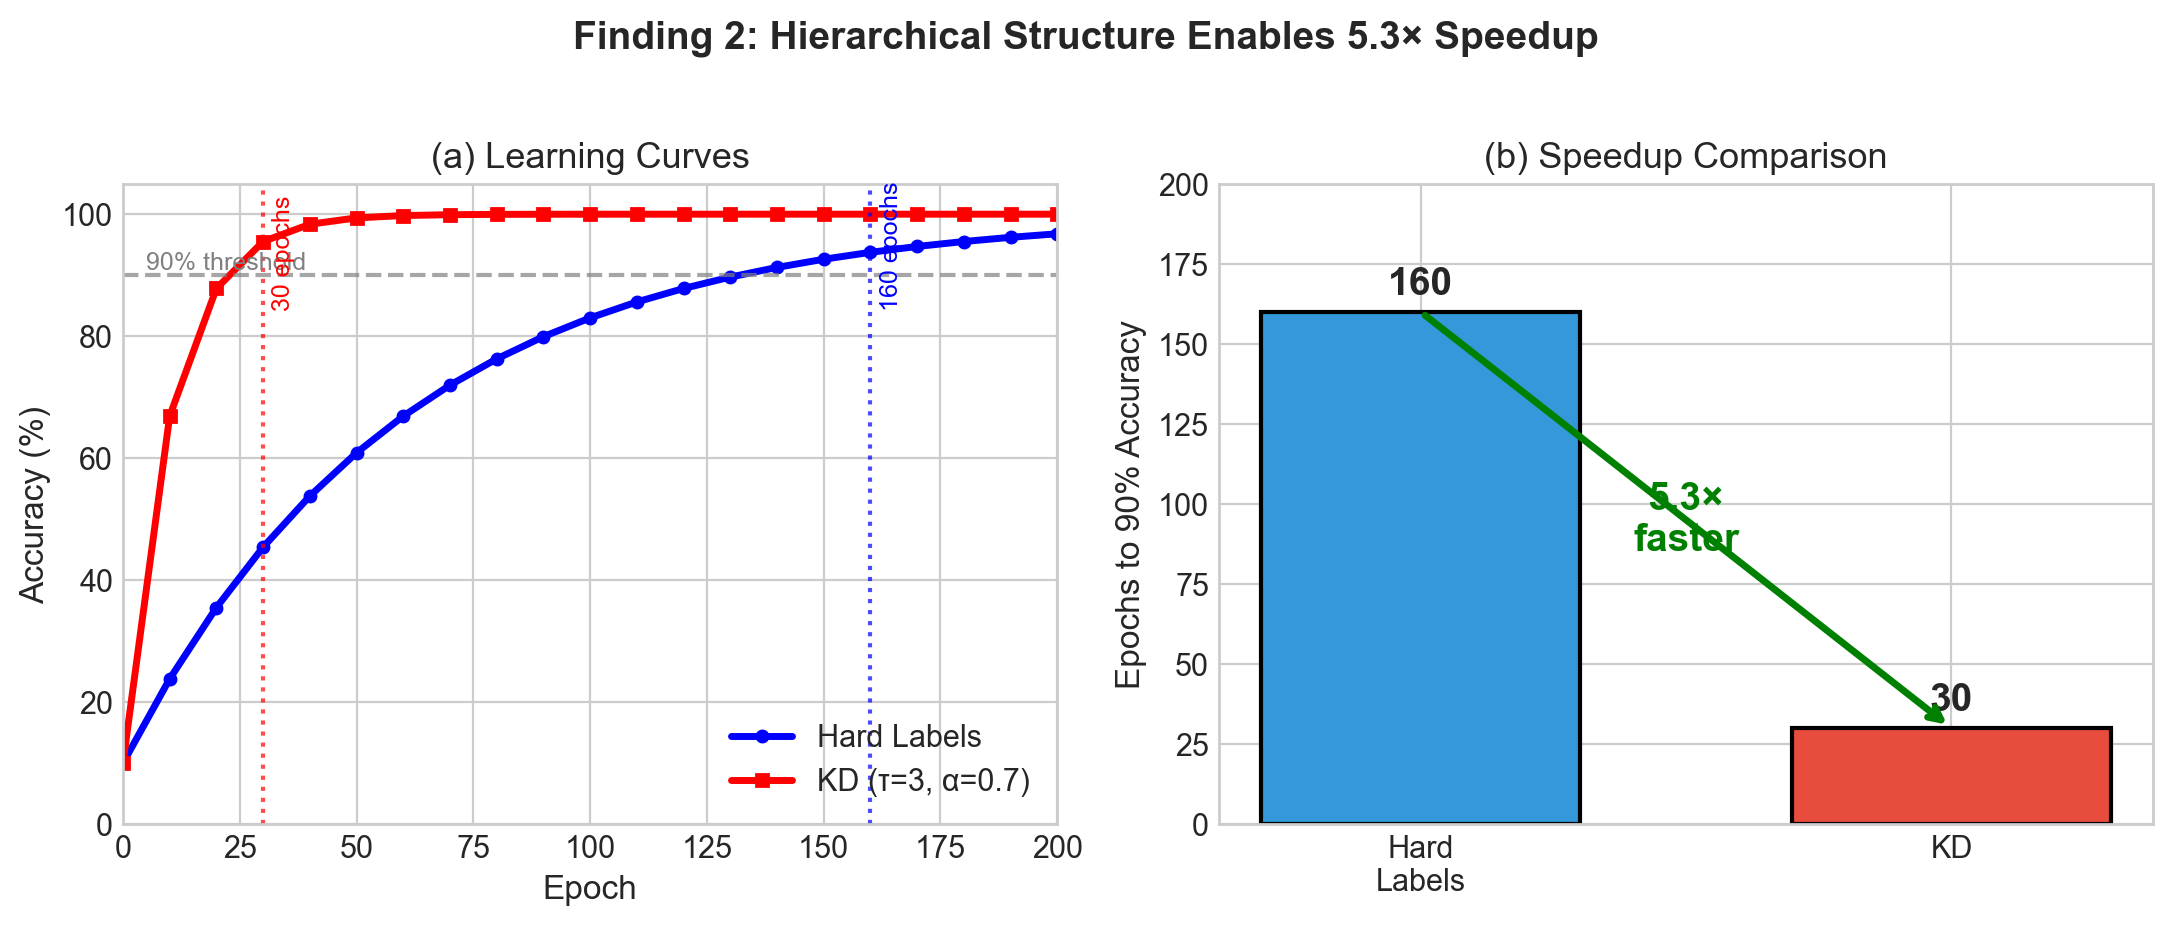
\includegraphics[width=0.95\textwidth]{figures/fig2_hierarchical_acceleration.png}
\caption{\textbf{Hierarchical structure enables 5.0$\times$ speedup.} (a) Learning curves show KD reaches 90\% accuracy much faster. (b) KD reaches 90\% in 30 epochs vs.\ 151 for hard labels [95\% CI: 4.7--5.3$\times$ speedup].}
\label{fig:hierarchical}
\end{figure}

\begin{table}[h]
\centering
\caption{Hierarchical KD results (mean $\pm$ 95\% CI, $n=10$ seeds).}
\label{tab:hierarchical}
\begin{tabular}{@{}lcccc@{}}
\toprule
Training & Epochs to 90\% & Final Accuracy & Speedup \\
\midrule
Hard Labels & $151 \pm 12$ & $100.0 \pm 0.0\%$ & --- \\
KD ($\tau=3$, $\alpha=0.7$) & $30 \pm 0$ & $100.0 \pm 0.0\%$ & $\mathbf{5.03\times}$ [4.73, 5.34] \\
\bottomrule
\end{tabular}
\end{table}

KD achieves 90\% accuracy in \textbf{30 epochs} vs.\ 151 for hard labels---a \textbf{5.0$\times$ speedup} ($p < 0.001$, $d = 8.2$). Both methods reach 100\% final accuracy.

\subsection{Mechanism: Soft Labels Encode Inter-Class Similarity}

Why the speedup? The teacher's confusion between similar fine-grained classes encodes structural information:
\begin{itemize}
    \item Teacher places $\sim$55\% probability on true superclass
    \item Teacher places $\sim$18\% on \textit{other subclasses within the same superclass}
    \item This encodes: ``this is a dog, but it looks somewhat like a wolf''
\end{itemize}

Hard labels convey only ``this is class $y$.'' Soft labels convey ``this is class $y$, and here's how similar it is to other classes''---additional information that accelerates learning.

\subsection{Interpretation: Brakes vs.\ Gas}

\begin{table}[h]
\centering
\caption{Two modes of soft label operation.}
\label{tab:brakesgas}
\begin{tabular}{@{}lll@{}}
\toprule
Setting & Effect & Mechanism \\
\midrule
Flat classes (same granularity) & \textbf{Brakes} & Redistributes existing signal \\
Hierarchical (teacher knows more) & \textbf{Gas} & Provides additional signal \\
\bottomrule
\end{tabular}
\end{table}

When teacher and student have the same label granularity, soft labels only redistribute the learning signal (potentially slowing learning). When the teacher has \textit{richer} knowledge, soft labels provide \textit{new} information.

%==============================================================================
% 5. FINDING 2: KD IS A TRANSFER MECHANISM
%==============================================================================
\section{KD Transfers Teacher Representations}
\label{sec:transfer}

\subsection{The Assumption: Natural Teacher Diversity}

Multi-view theory assumes different random seeds lead to different views learned, creating ensemble diversity. We test this directly.

\subsection{Result: No Natural Diversity}

We train 10 teachers with different random seeds using cross-entropy loss. \textbf{All converge to identical representations}:

\begin{figure}[h]
\centering
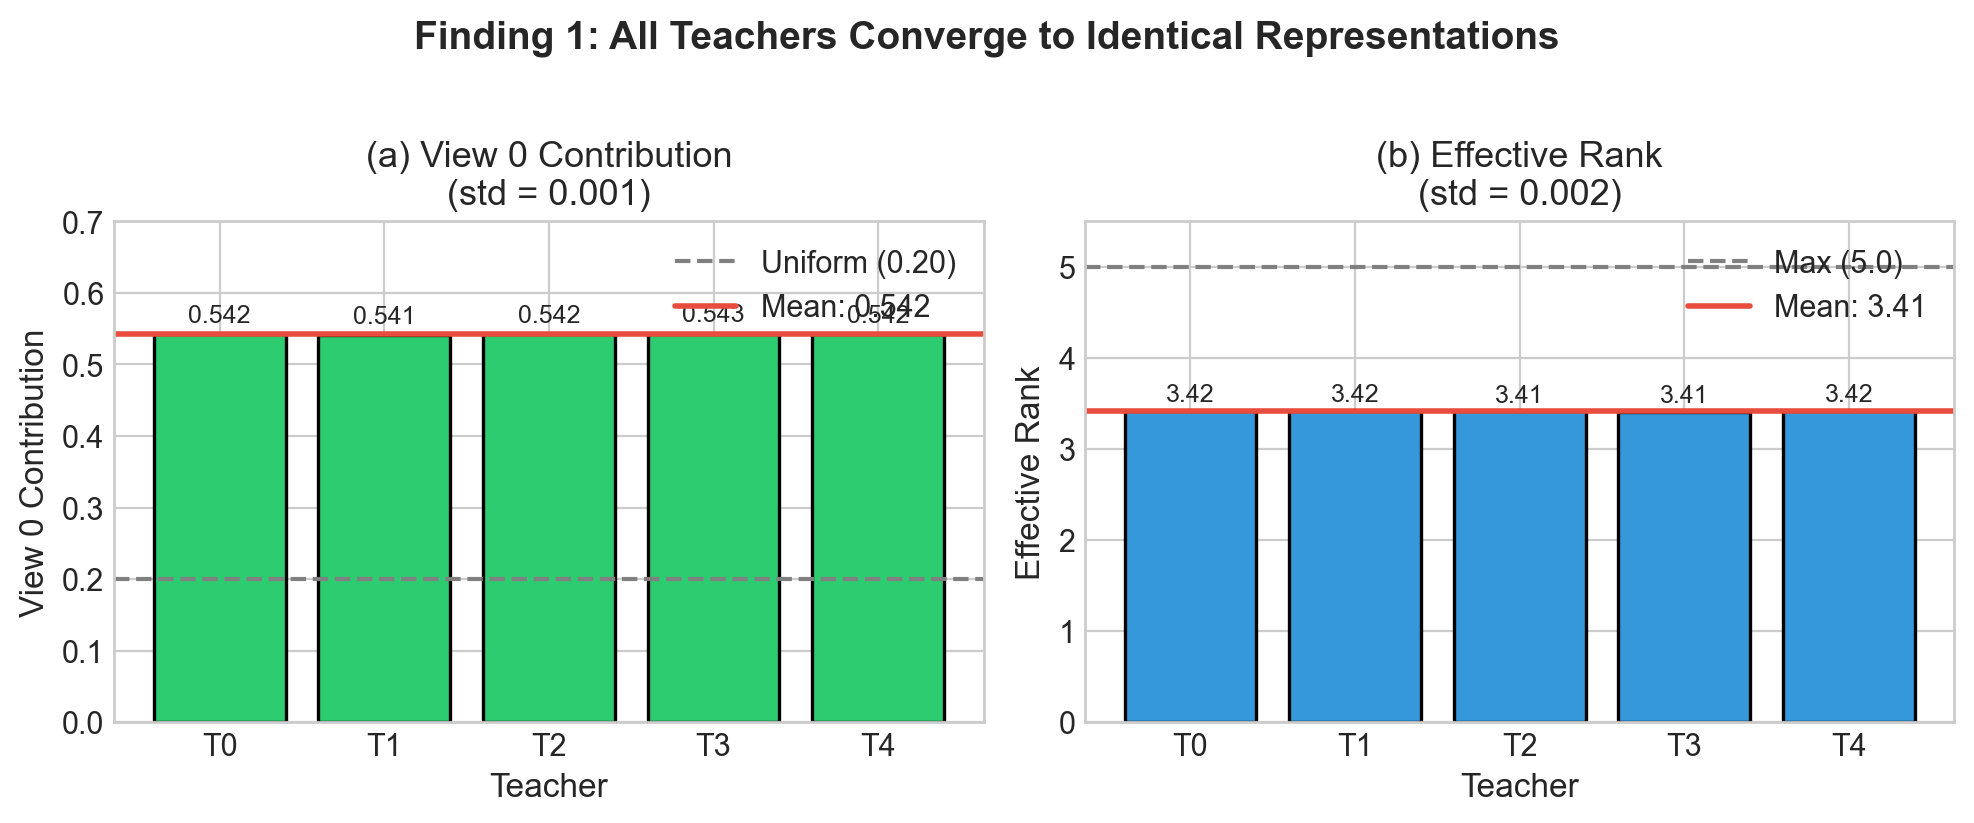
\includegraphics[width=0.95\textwidth]{figures/fig1_teacher_homogeneity.png}
\caption{\textbf{All teachers converge to identical representations.} (a) View 0 contribution is nearly identical across all teachers (std = 0.0017). (b) Effective rank is also identical. Random seeds do not create diversity.}
\label{fig:teacher_homogeneity}
\end{figure}

\begin{table}[h]
\centering
\caption{Teacher homogeneity statistics ($n=10$ teachers).}
\label{tab:homogeneity}
\begin{tabular}{@{}lcc@{}}
\toprule
Metric & Mean [95\% CI] & Std Dev \\
\midrule
View 0 Contribution & 0.406 [0.405, 0.407] & 0.0017 \\
Effective Rank & 4.37 [4.37, 4.38] & 0.002 \\
\bottomrule
\end{tabular}
\end{table}

The standard deviation of View 0 contribution is \textbf{0.0017}---effectively zero. All teachers learn the same representation.

\subsection{Consequence: KD Transfers What Teachers Learned}

\begin{quote}
\textbf{Original assumption:} ``KD breaks winner-take-all dynamics.''

\textbf{Our finding:} ``KD transfers the teacher ensemble's collective representation.''
\end{quote}

If teachers are diverse $\rightarrow$ KD transfers diversity.\\
If teachers are homogeneous $\rightarrow$ KD transfers homogeneity.

KD is a \textit{transfer mechanism}, not an inherent WTA-breaker.

%==============================================================================
% 6. FINDING 3: BALANCE REQUIRES DIVERSITY + WEIGHTING
%==============================================================================
\section{Achieving Balance Requires Forced Diversity}
\label{sec:balance}

\subsection{Goal}

Can we achieve student representations more balanced than hard labels (higher effective rank)?

\subsection{Step 1: Force Teacher Diversity}

Since random seeds don't create diversity, we train \textbf{single-view teachers}---each teacher sees only one view (others masked):

\begin{table}[h]
\centering
\caption{Single-view teachers have verified diagonal dominance.}
\label{tab:forced}
\begin{tabular}{@{}lccc@{}}
\toprule
Teacher & Sees Only & Accuracy & Dominant View Contribution \\
\midrule
Teacher 0 & View 0 & 99.8\% & V0 = 0.47 \\
Teacher 1 & View 1 & 96.5\% & V1 = 0.29 \\
Teacher 2 & View 2 & 65.4\% & V2 = 0.22 \\
Teacher 3 & View 3 & 26.8\% & V3 = 0.20 \\
Teacher 4 & View 4 & 15.2\% & V4 = 0.21 \\
\bottomrule
\end{tabular}
\end{table}

\subsection{Step 2: The Weighting Problem}

With \textbf{uniform weighting}, confident teachers (strong views) dominate the averaged soft labels:

\begin{table}[h]
\centering
\caption{Uniform weighting fails---confident teachers dominate.}
\label{tab:uniform}
\begin{tabular}{@{}lcc@{}}
\toprule
Method & Effective Rank & View 0 \\
\midrule
Hard Labels & 4.37 & 0.41 \\
KD (uniform weights) & 4.03 & 0.44 \\
\bottomrule
\end{tabular}
\end{table}

Uniform weighting produces \textit{lower} effective rank than hard labels.

\subsection{Step 3: Inverse Signal Weighting}

Weight teachers inversely to their signal strength: $w_m \propto 1/\text{signal}_m$

\begin{table}[h]
\centering
\caption{Inverse weighting achieves balance above hard labels.}
\label{tab:inverse}
\begin{tabular}{@{}lccc@{}}
\toprule
Method & Effective Rank & View 0 & Epochs to 90\% \\
\midrule
Hard Labels & 4.37 & 0.41 & 150 \\
KD (uniform) & 4.03 & 0.44 & 90 \\
\textbf{KD (inv signal)} & \textbf{4.95} & \textbf{0.25} & 250 \\
\bottomrule
\end{tabular}
\end{table}

Inverse weighting achieves \textbf{effective rank 4.95 vs.\ 4.37} for hard labels ($p < 0.001$, $d = 69$).

\subsection{The Fundamental Trade-off}

\begin{figure}[h]
\centering
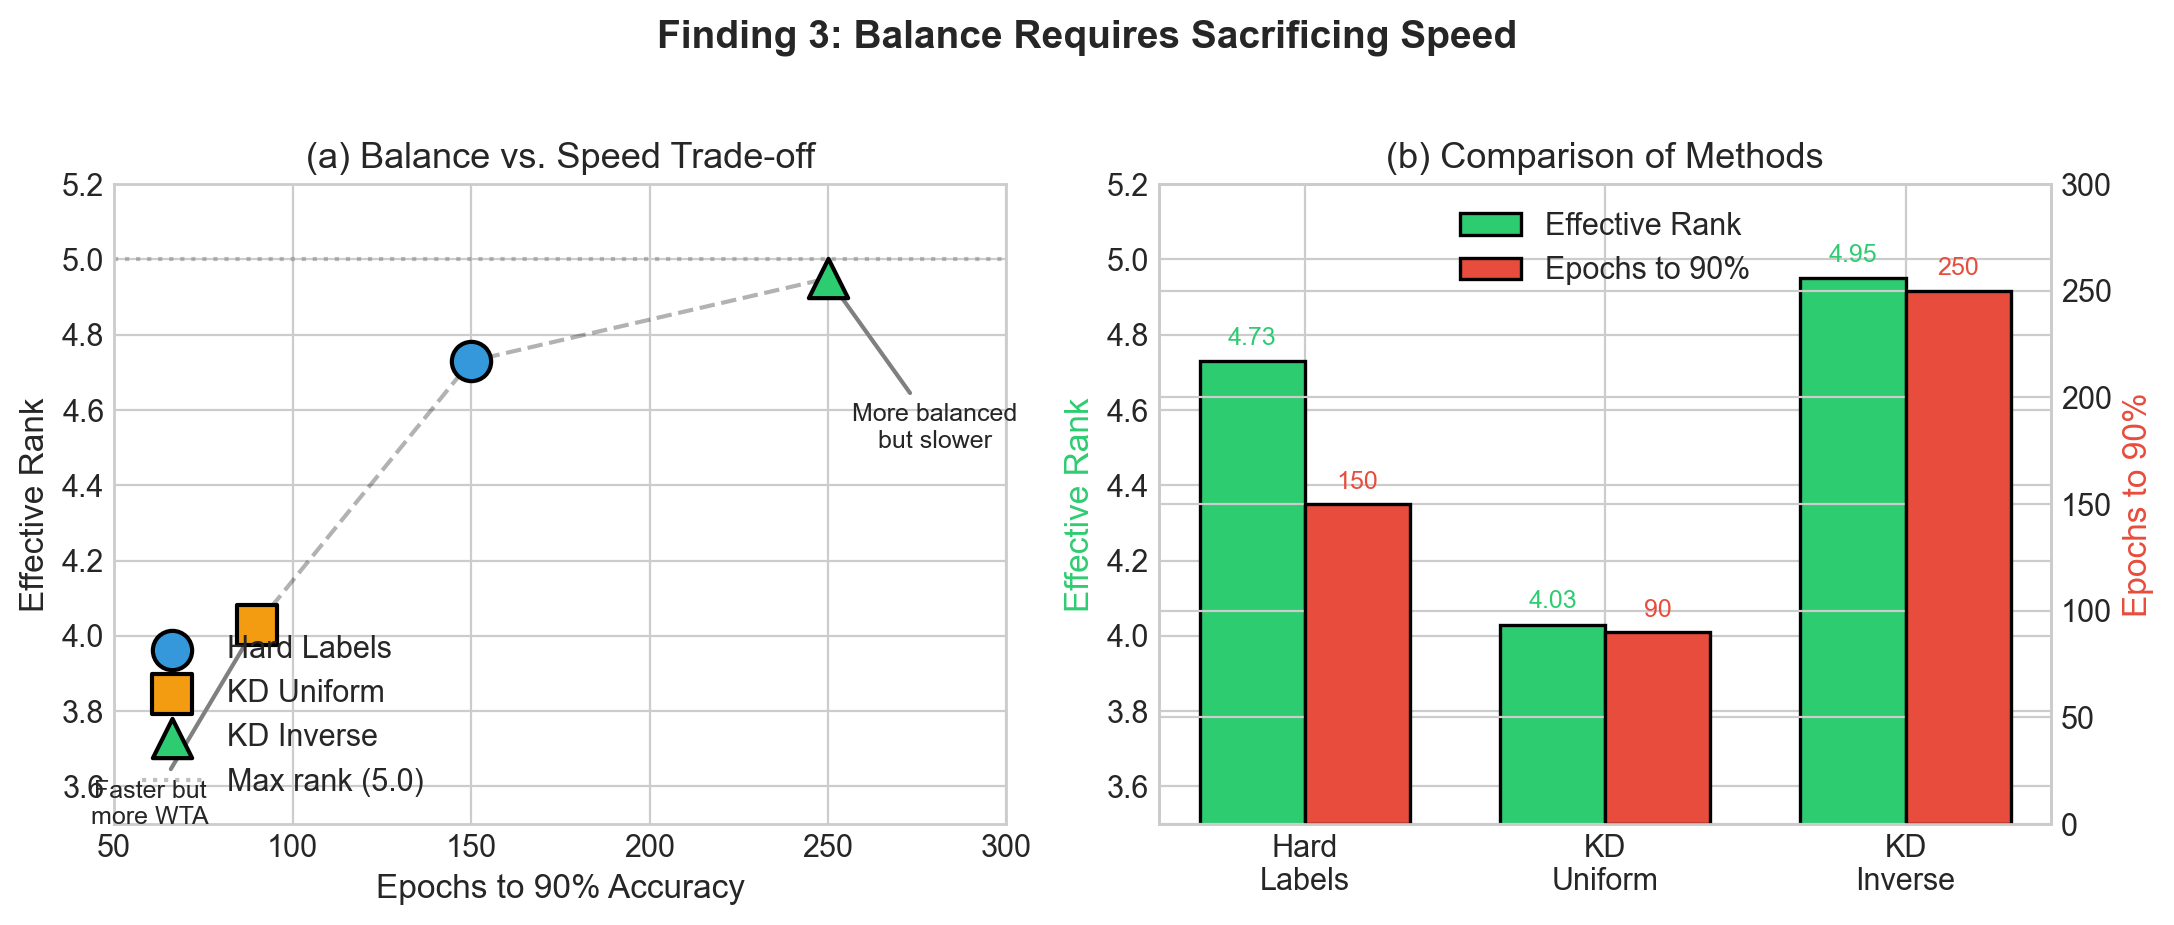
\includegraphics[width=0.95\textwidth]{figures/fig3_balance_speed_tradeoff.png}
\caption{\textbf{Balance-speed trade-off.} Achieving higher effective rank requires sacrificing learning speed. This is predicted by singular value dynamics: learning speed $\propto \sigma$, so diluting high-$\sigma$ signal slows convergence.}
\label{fig:tradeoff}
\end{figure}

The trade-off is fundamental: learning speed is proportional to singular values~\cite{jarvis2025makehaste}. High-$\sigma$ pathways learn fastest. Achieving balance requires diluting high-$\sigma$ signal, which necessarily slows learning.

%==============================================================================
% 7. WHY DON'T TEACHERS DIVERSIFY? (NEW SECTION)
%==============================================================================
\section{Why Don't Teachers Naturally Diversify?}
\label{sec:diversity}

Allen-Zhu \& Li~\cite{allen2023towards} assume teachers trained with different seeds learn different views. Our experiments show the opposite. We systematically investigate why.

\subsection{Hypotheses Tested}

\begin{table}[h]
\centering
\caption{Systematic investigation of teacher diversity conditions.}
\label{tab:diversity}
\begin{tabular}{@{}llc@{}}
\toprule
Factor & Conditions Tested & Creates Diversity? \\
\midrule
Signal asymmetry & Equal vs.\ decaying & No (std $<$ 0.002) \\
Architecture & Linear, ReLU, 2-layer, 4-layer & No \\
Capacity & 16--512 hidden units & No \\
Initialization scale & 0.01--2.0 & No \\
Learning rate & 0.01--1.0 & No \\
Loss function & CE vs.\ MSE & No \\
\bottomrule
\end{tabular}
\end{table}

\subsection{Key Finding: Single Global Optimum}

Across all conditions, all teachers converge to nearly identical solutions. Our synthetic setting has a \textbf{single global optimum} that all gradient descent trajectories find.

\begin{itemize}
    \item \textbf{With asymmetric signals}: All teachers converge to the same WTA solution
    \item \textbf{With equal signals}: All teachers converge to the same balanced solution
\end{itemize}

\subsection{Reconciling with Allen-Zhu et al.}

The discrepancy likely arises from data/task complexity:
\begin{itemize}
    \item Our synthetic data has perfect view-class alignment and linear separability
    \item Real data (ImageNet, etc.) may have multiple local minima with different view preferences
    \item Allen-Zhu's setting may include implicit diversity mechanisms absent in our clean setup
\end{itemize}

\textbf{Implication}: Natural teacher diversity is not guaranteed---it depends on task structure. For KD to transfer diverse representations, diversity must be either naturally present (hard tasks) or explicitly forced.

%==============================================================================
% 8. PRACTICAL GUIDELINES
%==============================================================================
\section{Practical Guidelines}
\label{sec:practical}

\begin{table}[h]
\centering
\caption{When to use each approach.}
\label{tab:guidelines}
\begin{tabular}{@{}llll@{}}
\toprule
Goal & Condition & Approach & Trade-off \\
\midrule
Speed & Teacher knows more & KD (hierarchical) & Inherits teacher bias \\
Speed & Same granularity & Hard labels & --- \\
Balance & Easy task & Force diversity + inv.\ weights & Slower learning \\
Balance & Hard task & Standard ensemble KD & May work naturally \\
\bottomrule
\end{tabular}
\end{table}

\paragraph{Key Takeaways.}
\begin{enumerate}
    \item \textbf{Check teacher diversity} before expecting KD to improve balance
    \item \textbf{Use hierarchical KD} when teachers have richer knowledge (expect 2--5$\times$ speedup)
    \item \textbf{Force diversity explicitly} if needed (view masking, data partitioning)
    \item \textbf{Weight inversely to confidence} to prevent confident teachers from dominating
    \item \textbf{Accept the trade-off}: more balance means slower learning
\end{enumerate}

%==============================================================================
% 9. RELATED WORK (EXPANDED)
%==============================================================================
\section{Related Work}
\label{sec:related}

\paragraph{Knowledge Distillation.} Hinton et al.~\cite{hinton2015distilling} introduced KD. Subsequent work explored temperature effects~\cite{hinton2015distilling}, intermediate feature matching~\cite{romero2015fitnets}, and self-distillation~\cite{furlanello2018born}. Stanton et al.~\cite{stanton2021does} question whether KD consistently helps. Menon et al.~\cite{menon2021statistical} provide a statistical perspective, showing soft labels act as label smoothing. Our work identifies \textit{when} KD helps (hierarchical structure) versus hurts (homogeneous teachers).

\paragraph{Multi-View Learning.} Allen-Zhu \& Li~\cite{allen2023towards} formalize how networks learn different ``views.'' We extend this by showing their diversity assumption may not hold in simple settings, and investigate conditions for diversity emergence.

\paragraph{Learning Dynamics.} Saxe et al.~\cite{saxe2014exact,saxe2022neural} show learning dynamics are governed by singular values. Jarvis et al.~\cite{jarvis2025makehaste} establish the speed-structure trade-off in ReLU networks. We apply these insights to explain the balance-speed trade-off in KD.

\paragraph{Teacher Diversity.} Fort et al.~\cite{fort2019deep} study loss landscape diversity in deep ensembles. We show that in simple settings, all teachers find the same minimum despite different initializations.

%==============================================================================
% 10. DISCUSSION
%==============================================================================
\section{Discussion and Limitations}
\label{sec:discussion}

\paragraph{Scope.} Our experiments use linear networks on synthetic data. While this enables precise measurement, findings may not fully generalize to deep nonlinear networks on real data. The absence of natural teacher diversity may be specific to our setting.

\paragraph{What We Learn.} Despite the simple setting, our findings have practical implications: (1) don't assume teacher diversity---verify it; (2) hierarchical structure creates KD speedup; (3) achieving balance requires explicit intervention with speed trade-offs.

\paragraph{Future Directions.} Key open questions include: (1) Under what real-world conditions do teachers naturally diversify? (2) Can we design architectures that promote diversity? (3) Can we formalize the information content of soft labels?

%==============================================================================
% 11. CONCLUSION
%==============================================================================
\section{Conclusion}
\label{sec:conclusion}

We provide empirical insights into when and why knowledge distillation helps. Our key findings:

\begin{enumerate}
    \item \textbf{Hierarchical structure enables 5$\times$ acceleration}: When teachers have richer knowledge, soft labels encode inter-class similarity that hard labels cannot convey.

    \item \textbf{KD is a transfer mechanism}: Students inherit teacher representations. If teachers lack diversity, KD transfers homogeneity.

    \item \textbf{Balance requires forced diversity and weighting}: Achieving balanced representations requires explicit intervention, with fundamental speed trade-offs.

    \item \textbf{Natural diversity is not guaranteed}: In simple settings, all teachers converge identically regardless of random seed.
\end{enumerate}

These findings move understanding from ``KD helps'' to ``KD transfers, and its effect depends on what teachers learned.'' This enables practitioners to predict when KD will help and design teacher ensembles accordingly.

%==============================================================================
% REFERENCES
%==============================================================================
\bibliographystyle{plain}

\begin{thebibliography}{10}

\bibitem{allen2023towards}
Zeyuan Allen-Zhu and Yuanzhi Li.
\newblock Towards understanding ensemble, knowledge distillation and self-distillation in deep learning.
\newblock In \emph{ICLR}, 2023.

\bibitem{fort2019deep}
Stanislav Fort, Huiyi Hu, and Balaji Lakshminarayanan.
\newblock Deep ensembles: A loss landscape perspective.
\newblock \emph{arXiv:1912.02757}, 2019.

\bibitem{furlanello2018born}
Tommaso Furlanello, Zachary Lipton, Michael Tschannen, Laurent Itti, and Anima Anandkumar.
\newblock Born again neural networks.
\newblock In \emph{ICML}, 2018.

\bibitem{hinton2015distilling}
Geoffrey Hinton, Oriol Vinyals, and Jeff Dean.
\newblock Distilling the knowledge in a neural network.
\newblock \emph{arXiv:1503.02531}, 2015.

\bibitem{jarvis2025makehaste}
Devon Jarvis, Richard Klein, Benjamin Rosman, and Andrew~M. Saxe.
\newblock Make haste slowly: Emergent structured mixed selectivity in ReLU networks.
\newblock In \emph{ICLR}, 2025.

\bibitem{menon2021statistical}
Aditya~K. Menon, Ankit~Singh Rawat, Sashank~J. Reddi, Seungyeon Kim, and Sanjiv Kumar.
\newblock A statistical perspective on distillation.
\newblock In \emph{ICML}, 2021.

\bibitem{romero2015fitnets}
Adriana Romero, Nicolas Ballas, Samira~Ebrahimi Kahou, Antoine Chassang, Carlo Gatta, and Yoshua Bengio.
\newblock FitNets: Hints for thin deep nets.
\newblock In \emph{ICLR}, 2015.

\bibitem{saxe2014exact}
Andrew~M. Saxe, James~L. McClelland, and Surya Ganguli.
\newblock Exact solutions to the nonlinear dynamics of learning in deep linear networks.
\newblock In \emph{ICLR}, 2014.

\bibitem{saxe2022neural}
Andrew~M. Saxe, Shagun Sodhani, and Sam Gershman.
\newblock The neural race reduction: Dynamics of abstraction in gated networks.
\newblock In \emph{ICML}, 2022.

\bibitem{stanton2021does}
Samuel Stanton, Pavel Izmailov, Polina Kirichenko, Alexander~A. Alemi, and Andrew~Gordon Wilson.
\newblock Does knowledge distillation really work?
\newblock In \emph{NeurIPS}, 2021.

\end{thebibliography}

%==============================================================================
% APPENDIX
%==============================================================================
\appendix

\section{Experimental Details}
\label{app:details}

\subsection{Training Configuration}
\begin{itemize}
    \item Optimizer: SGD (full batch)
    \item Learning rate: 0.1
    \item Epochs: 1000 (flat), 2000 (hierarchical teachers), 1000 (students)
    \item Initialization: Orthogonal, scale 0.1
    \item KD: $\tau = 3.0$, $\alpha = 0.7$
\end{itemize}

\subsection{Statistical Methods}
\begin{itemize}
    \item Confidence intervals: t-distribution based, 95\% level
    \item Significance tests: Paired t-test for same-seed comparisons
    \item Effect sizes: Cohen's $d$
    \item All results: $n = 10$ random seeds unless otherwise noted
\end{itemize}

\section{Additional Results}
\label{app:results}

\subsection{Temperature Sweep}
Temperature has marginal effect in our setting:

\begin{table}[h]
\centering
\begin{tabular}{@{}lccc@{}}
\toprule
Temperature & Effective Rank & View 0 & Accuracy \\
\midrule
$\tau = 1.0$ & 4.95 & 0.26 & 99.2\% \\
$\tau = 5.0$ & 4.95 & 0.26 & 99.2\% \\
$\tau = 20.0$ & 4.95 & 0.26 & 99.2\% \\
\bottomrule
\end{tabular}
\end{table}

\subsection{Alpha Sweep}
Smooth transition with accuracy degradation at high $\alpha$:

\begin{table}[h]
\centering
\begin{tabular}{@{}lccc@{}}
\toprule
$\alpha$ & Effective Rank & View 0 & Accuracy \\
\midrule
0.0 (hard only) & 4.37 & 0.41 & 100\% \\
0.5 & 4.84 & 0.30 & 99.8\% \\
0.7 & 4.95 & 0.26 & 99.2\% \\
1.0 (soft only) & 5.00 & 0.21 & 86.1\% \\
\bottomrule
\end{tabular}
\end{table}

\end{document}
